%\subsection{Preliminaries}
\subsection{What You Should Know}

\begin{frame}{\insertsubsection{}}
	\leftorright{
		\mynote{Fundamentals of Software Engineering}{
			\begin{itemize}
				\item object-oriented programming
				\item design patterns
				\item UML class diagrams
				\item modularity
				\item development processes
				\item \todots
			\end{itemize}
		}
	}{
		\mynote{Fundamentals of Theoretical Computer Science}{
			\begin{itemize}
				\item set theory
				\item propositional logic
				\item complexity theory
				\item abstract syntax trees
				\item \todots
			\end{itemize}
		}

		\mynote{Exercise}{
			solid programming skills in Java
		}
	}
\end{frame}

%\subsection{Course Overview}
\subsection{What You Will Learn}

\begin{frame}{\insertsubsection{}}
	\leftorright{
		\mynote{Part I: Ad-Hoc Approaches for Variability}{
			\begin{enumerate}
				\item Introduction
				\item Runtime Variability and Design Patterns
				\item Compile-Time Variability with Clone-and-Own
			\end{enumerate}
		}
		\mynote{\small Part II: Modeling and Implementing Product Lines}{
			\begin{enumerate}
				\setcounter{enumi}{3}
				\item Feature Modeling
				\item Techniques for Compile-Time Features
				\item Techniques for Modular Variability
				\item Language-Based Techniques
				\item Development Process
			\end{enumerate}
		}
	}{
		\mynote{Part III: Quality Assurance and Maintenance}{
			\begin{enumerate}
				\setcounter{enumi}{8}
				\item Feature Interactions
				\item Product-Line Analyses
				\item Product-Line Testing
				\item Evolution and Maintenance
			\end{enumerate}
		}
	}
\end{frame}

%\subsection{Literature and Tool Support}
\subsection{What You Might Need}

\begin{frame}{\insertsubsection{}}
	\leftorright{
		\myexampletight{Recommended Literature for Lecture \& Exercise}{
			\centering
			\parbox{0.49\linewidth}{
				\centering
				\href{http://link.springer.com/book/10.1007/978-3-642-37521-7}{
\includegraphics[width=\linewidth]{cover-fospl}}
				\emph{theory-focused}
			}
			\parbox{0.475\linewidth}{
				\centering
				\href{http://www.springer.com/de/book/9783319614427}{
\includegraphics[width=\linewidth]{cover-featureide}}
				\emph{practice-oriented}
			}
		}
	}{
		\myexampletight{Recommended Tool Support for the Exercise}{
			\centering
			\href{https://featureide.github.io/}{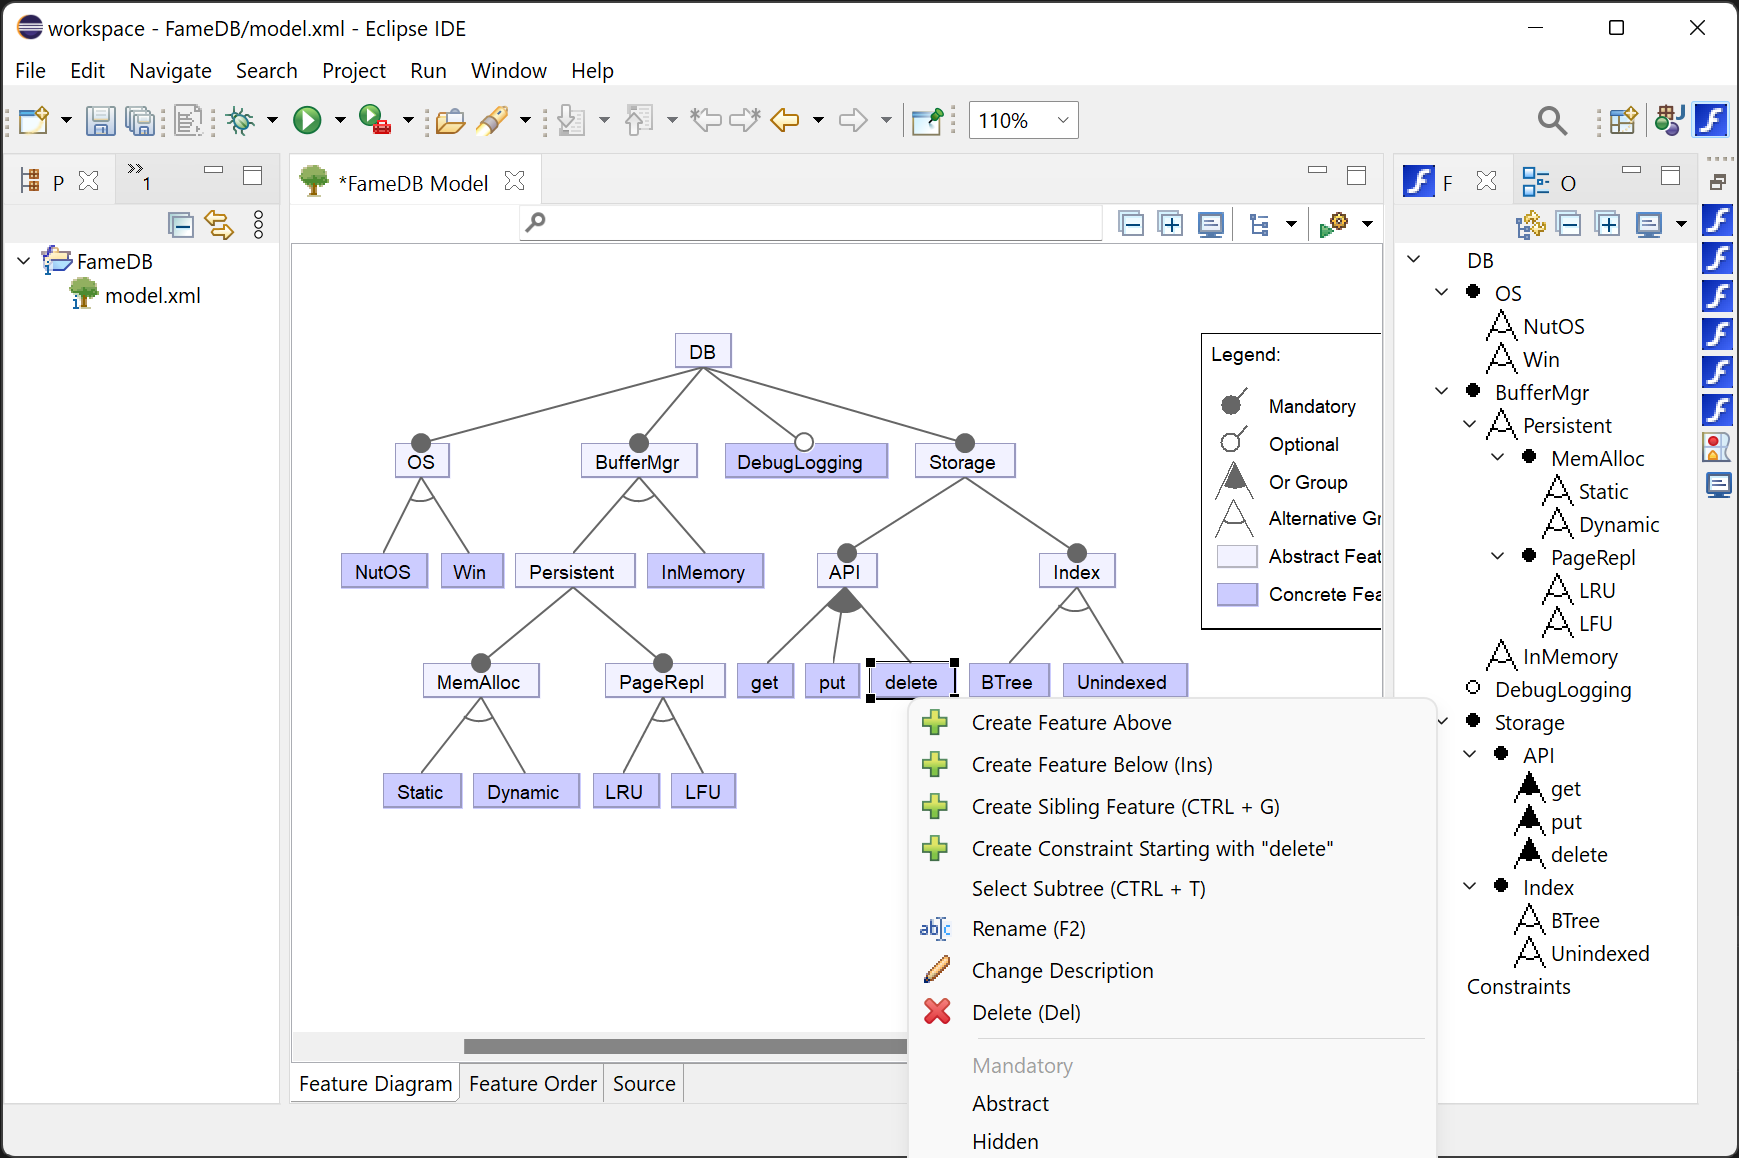
\includegraphics[width=\linewidth]{featureide-feature-model-editor.png}}\\[.5ex]
			\href{https://featureide.github.io/}{
\includegraphics[width=0.25\linewidth]{featureide-logo.png}}
		}
	}
\end{frame}